% Informe TP — Maestría en IA, Visión y Percepción Computarizada
% Compilar: pdflatex informe_paper.tex  (desde la carpeta docs/)
\documentclass[conference]{IEEEtran}

\usepackage[utf8]{inputenc}
\usepackage[T1]{fontenc}
\usepackage[spanish]{babel}
\usepackage{amsmath,amssymb}
\usepackage{graphicx}
\usepackage{booktabs}
\usepackage{hyperref}
\usepackage{subcaption}
\usepackage{xcolor}
\usepackage{url}

\graphicspath{{../results_dann/}{../statistical_analysis/}}

% ---- Metadatos ---------------------------------------------------------------
\title{Clasificación de TEA en rs-fMRI mediante CNN 2D\\
       con Generalización Adversarial de Dominio (DANN)}

\author{
  \IEEEauthorblockN{Leandro Carcagno,\ Sebastián Mesch Henriques}
  \IEEEauthorblockA{Maestría en Inteligencia Artificial\\
    Universidad de San Andrés (UDESA), Argentina}
}

\begin{document}
\maketitle

% ---- Abstract ----------------------------------------------------------------
\begin{abstract}
Presentamos un pipeline reproducible de clasificación binaria
\emph{Trastorno del Espectro Autista (ASD) vs.\ Control Típico (TC)}
sobre datos de resonancia magnética funcional en reposo (rs-fMRI) del
dataset público ABIDE~I. El rs-fMRI es un dato 4D que registra, voxel por voxel (las 3 dimensiones espaciales), la evolución temporal de la actividad cerebral mientras la persona está en reposo.
El enfoque convierte estos estudios en tensores 2D multicanal ($6{\times}64{\times}64$). Para ello, primero colapsa la dimensión temporal calculando las métricas fALFF y ReHo para cada voxel, y luego extrae cortes sagital, coronal y axial seleccionados por máximo
\emph{Cohen's\,$d$} inter-grupo. Una CNN liviana (29\,027 parámetros)
con entrenamiento adversarial de dominio (DANN, \emph{Gradient Reversal
Layer}) aprende representaciones invariantes a los 18 sitios de
adquisición, y se evalúa en dos sitios no vistos (PITT, OLIN,
$n\!=\!90$). El modelo con DANN obtiene AUC\,=\,0.588 frente a
AUC\,=\,0.552 del modelo sin DANN, con una mejora en \emph{balanced
accuracy} de $+$6.6\,pp. Los resultados son consistentes con la
hipótesis de que la invarianza de dominio adversarial mejora la
generalización multi-sitio, aunque la diferencia no alcanza
significancia estadística con el tamaño muestral actual de test;
se discuten las limitaciones y las extensiones requeridas
(\emph{leave-one-site-out}, tests pareados de DeLong).
\end{abstract}

\begin{IEEEkeywords}
autismo, rs-fMRI, ABIDE, domain adaptation, DANN, CNN, fALFF, ReHo,
generalización multi-sitio, neuroimagen computacional
\end{IEEEkeywords}

% ---- 1. Introducción ---------------------------------------------------------
\section{Introducción}

El Trastorno del Espectro Autista (ASD) se diagnostica clínicamente
mediante observación conductual e instrumentos estructurados (ADOS,
ADI-R). La búsqueda de biomarcadores objetivos en neuroimagen es un
campo activo: el consorcio \emph{Autism Brain Imaging Data Exchange}
(ABIDE) pone a disposición datos de rs-fMRI de más de 1\,000 sujetos
en más de 20 sitios de adquisición~\cite{diMartino2014}, habilitando
estudios a gran escala.

El estado del arte en clasificación ABIDE tiende a usar matrices de
conectividad funcional~\cite{heinsfeld2018}. Este trabajo adopta un
encuadre alternativo basado en \emph{visión por computadora}: generar mapas
paramétricos voxel-wise (fALFF~\cite{zou2008}, ReHo~\cite{zang2004}), realizar cortes 2D de los mismos y realizar una clasificación final con una CNN. Este enfoque
es más interpretable.

Superado el problema de generar imágenes 2D que sirvan como input al modelo, se tiene como segundo desafío el \emph{domain shift} multicentro: distintos
resonadores, intensidades de campo e implementaciones de secuencias
introducen variaciones sistemáticas ajenas a la neuropatología. Para
combatirlo implementamos la maquinaria DANN~\cite{ganin2016}, donde
una \emph{Gradient Reversal Layer} (GRL) fuerza al extractor de
características a ser invariante al sitio de origen mientras maximiza
la discriminación diagnóstica.

Las contribuciones del trabajo son:
\begin{itemize}
  \item Pipeline reproducible ABIDE\,$\to$\,PNG\,$\to$\,CNN con control
        riguroso de \emph{data leakage} (split por sujeto, evaluación
        out-of-distribution, fenotipos excluidos del modelo).
  \item Comparación controlada DANN vs.\ sin-DANN: misma arquitectura,
        mismos hiperparámetros, mismo estado de inicialización aleatoria.
  \item Análisis estadístico de los resultados.
\end{itemize}

% ---- 2. Datos ----------------------------------------------------------------
\section{Datos}

\subsection{Cohorte ABIDE PCP}

Utilizamos derivados preprocesados del \emph{Preprocessed Connectomes
Project} (PCP) de ABIDE\,I~\cite{craddock2013}.
Se tienen 1\,035 sujetos procesados exitosamente
(505 ASD / 530 TC), provenientes de 20 sitios diferentes. El conjunto de test
son los sitios PITT ($n\!=\!56$) y OLIN ($n\!=\!34$), 90 sujetos en
total (48 ASD / 42 TC), reservados completamente.

\subsection{Mapas Derivados}

A partir de los estudios, se realizan dos mapas paramétricos por sujeto:

\begin{itemize}
  \item \textbf{fALFF}~\cite{zou2008}: registra la amplitud relativa de las
        fluctuaciones de baja frecuencia en la señal BOLD, normalizada
        por el espectro total.
  \item \textbf{ReHo}~\cite{zang2004}: representa la homogeneidad regional de la
        serie temporal de un voxel respecto de sus 26 vecinos (coeficiente
        de concordancia de Kendall $W$).
\end{itemize}

Para comprimir la dimensión temporal, se toma el valor medio que registró cada voxel a lo largo del estudio. De este paso se obtienen dos representaciones tridimensionales de cada cerebro.

Los volúmenes están en espacio \textbf{MNI152 3\,mm} (grilla
$61{\times}73{\times}61$ voxels), garantizando que el mismo índice de
voxel corresponda aproximadamente a la misma región anatómica entre
sujetos.

\subsection{Selección de Cortes (VBM-like)}

A fin de no generar un modelo demasiado complejo y limitar la dimensión del input, se decidió que el modelo reciba 6 imágenes como tensor de ingreso. Tres imágenes provendrán de la representación del fALFF, y tres del ReHo.

De cada representación se obtendrá un corte sagital, otro coronal y uno axial.
Debe decidirse entonces dónde realizar cada corte, y para ello se utiliza el 
\emph{Cohen's\,$d$} voxel-wise entre las muestras ASD\,y \,TC sobre el conjunto de
entrenamiento (PITT y OLIN excluidos). La d de Cohen es una medida estadística del tamaño del efecto que indica la magnitud de la diferencia entre dos medias, expresada en desviaciones estándar. Lo que se está haciendo en definitiva es registrar si hay una diferencia sustancial en el valor medio de cada voxel entre sujetos ASD y TC. Se seleccionan el plano sagital, coronal y axial de mayor
media de $|d|$ dentro de la máscara cerebral~\cite{muellerRissman2015}.

Los índices resultantes son:
\textbf{fALFF}: sagital\,=\,10, coronal\,=\,8, axial\,=\,17;
\textbf{ReHo}: sagital\,=\,30, coronal\,=\,10, axial\,=\,48.

Es importante destacar que los efectos ganadores tienen $|d|\approx0.07$--$0.09$, valores
convencionalmente despreciables (Suele decirse que un Cohen de valor pequeño es de $\approx0.2$). Esto
anticipa la dificultad del problema y es coherente con los AUC
obtenidos. Estos resultados adelantan que las imágenes no parecieran incluir información relevante y con claras diferencias entre los dos grupos en análisis.


Los 6 cortes por sujeto se apilan como tensor
$\mathbf{X} \in \mathbb{R}^{6 \times 64 \times 64}$,
redimensionados con interpolación bilineal. 

% ---- 3. Métodos --------------------------------------------------------------
\section{Métodos}

\subsection{Arquitectura ASD\_DANN}

La red consta de un \textbf{extractor de características compartido} y
dos cabezales competitivos:

\begin{figure}[t]
  \centering
  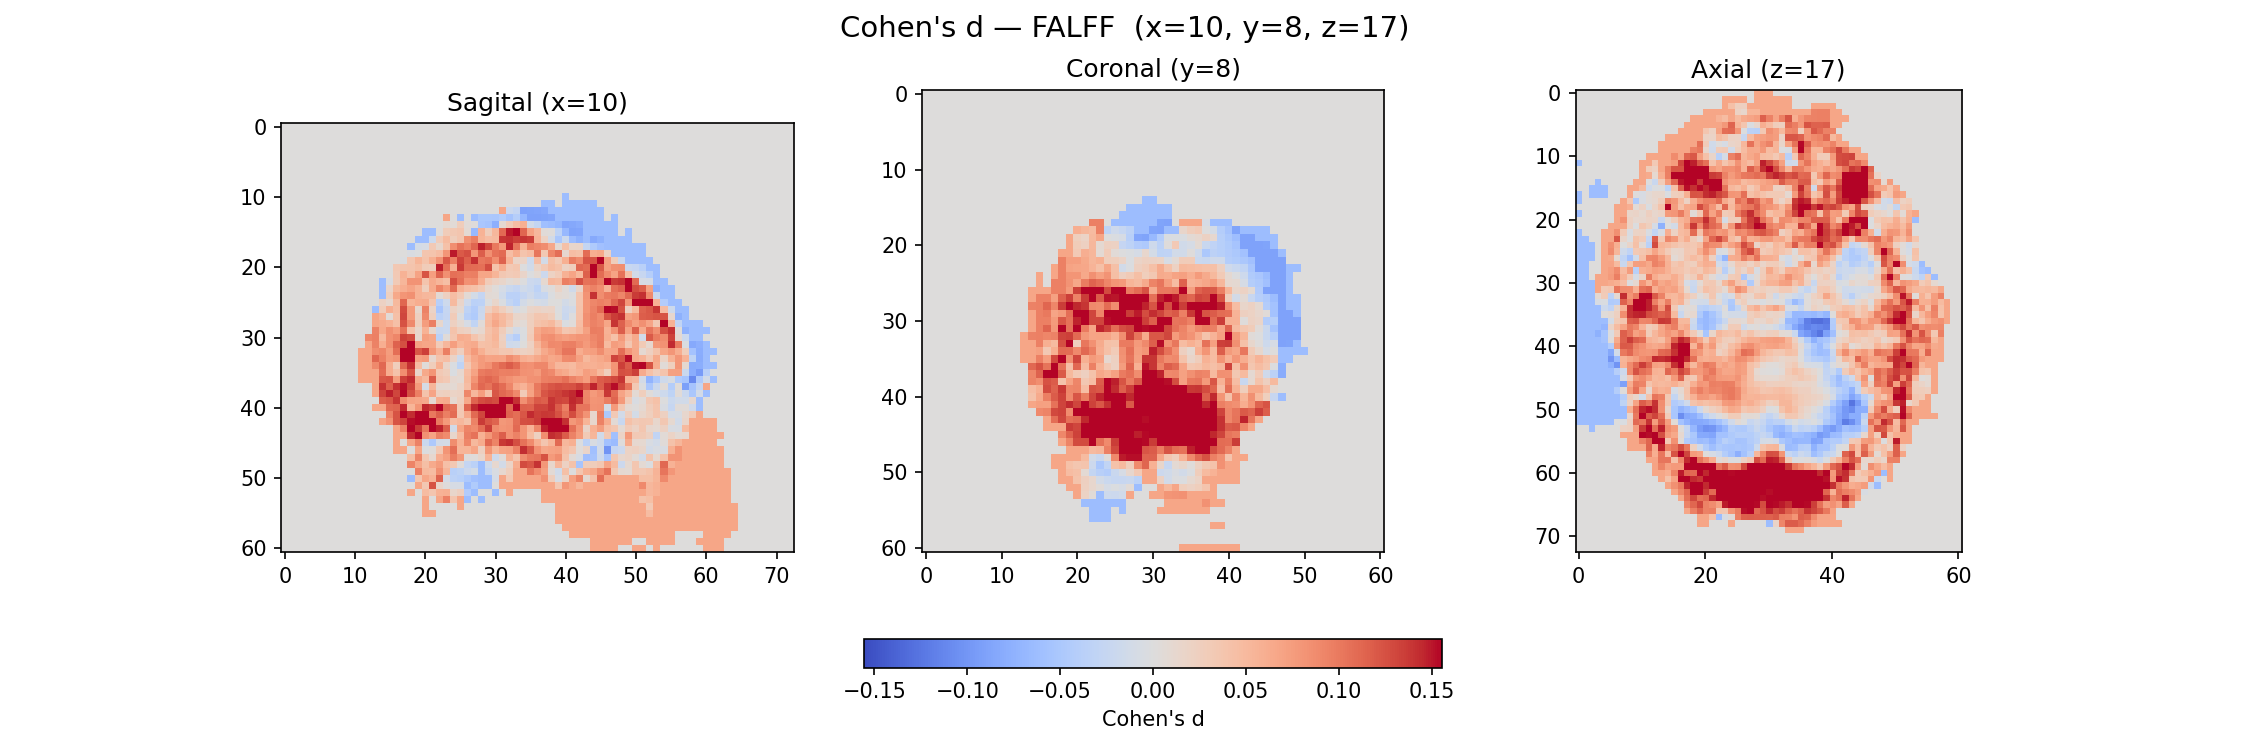
\includegraphics[width=\columnwidth]{optimal_tmap_falff.png}
  \caption{T-map fALFF (ASD vs.\ TC) en el plano coronal óptimo
           ($k\!=\!8$). Intensidades próximas al blanco indican
           mayor $|d|$; la señal es débil y dispersa, lo que es
           representativo del problema.}
  \label{fig:tmap}
\end{figure}

\begin{itemize}
  \item \textbf{Extractor}: tres bloques
        Conv2D\,$3{\times}3$\,+\,BN\,+\,ReLU\,+\,MaxPool\,+\,Dropout2D
        ($p\!=\!0.018$) con $6{\to}16{\to}32{\to}64$ canales,
        seguidos de \emph{Global Average Pooling} (GAP) a un vector
        de 64 dimensiones. El GAP reduce la complejidad paramétrica
        y actúa como regularizador estructural.
  \item \textbf{Cabezal diagnóstico}:
        $64{\to}32{\to}1$ (logit ASD vs.\ TC).
  \item \textbf{Cabezal de dominio (GRL)}:
        $64{\to}32{\to}n_\text{sitios}$ precedido por la GRL que
        multiplica el gradiente de dominio por $-\alpha$ durante el
        backward, impidiendo que el extractor capture la firma del
        scanner.
\end{itemize}

Total: \textbf{29\,027 parámetros}. El tamaño reducido es deliberado
dado el tamaño muestral ($\approx$\,800 sujetos de entrenamiento).

\textbf{Modo sin DANN}: se fija $\alpha\!=\!0$, anulando el gradiente
adversarial. La arquitectura, la inicialización y el estado RNG son
idénticos a los del modelo con DANN, lo que hace la comparación
perfectamente controlada.

\subsection{Función de Pérdida}

\begin{equation}
  \mathcal{L} = \mathcal{L}_\text{tarea} + \mathcal{L}_\text{dominio}
\end{equation}

donde $\mathcal{L}_\text{tarea}$ es BCE con \emph{label smoothing}
simétrico ($s\!=\!0.046$):
\begin{equation}
  \hat{y} = y\,(1-s) + 0.5\,s
\end{equation}
y $\mathcal{L}_\text{dominio}$ es entropía cruzada sobre los 18 sitios
de train/val. El efecto adversarial actúa a través del GRL, no
mediante signo negativo en la suma.

En definitiva, el entrenamiento consiste en una iteración de los parámetros para producir representaciones buenas para el cabezal diagnóstico y, simultáneamente, malas para el cabezal de dominio. Esa representación mala se logra invirtiendo su gradiente con la GRL, de modo que el ajuste se de cada paso se realiza yendo en la dirección "contraria" a la que optimizaría al cabezal. 

El resultado es que las características que salen del extracto sean discriminativas para ASD/TC pero invariantes al scanner.

\subsection{Entrenamiento}

Los hiperparámetros se buscaron con Optuna (sampler TPE, maximizando
val\,AUC):

\begin{table}[h]
  \centering
  \caption{Hiperparámetros finales (desde \texttt{config.toml})}
  \label{tab:hparams}
  \begin{tabular}{lc}
    \toprule
    Hiperparámetro & Valor \\
    \midrule
    Learning rate (AdamW) & $3.18\times10^{-4}$ \\
    Batch size            & 64 \\
    DANN $\alpha$         & 0.212 \\
    Dropout (Dropout2D)   & 0.018 \\
    Label smoothing       & 0.046 \\
    Epochs máximos        & 200 \\
    Patience (early stop) & 55 \\
    Scheduler             & ReduceLROnPlateau \\
    \bottomrule
  \end{tabular}
\end{table}

El split es:
\textbf{test} = PITT + OLIN (90 sujetos, completamente excluidos);
\textbf{train/val} = 85/15\% del resto, estratificado por
(diagnóstico, sitio). \emph{Early stopping} por val\,AUC;
\texttt{WeightedRandomSampler} para equilibrar clases en cada batch.

% ---- 4. Resultados -----------------------------------------------------------
\section{Resultados}

\subsection{Métricas en Test (PITT + OLIN)}

La Tabla~\ref{tab:results} compara ambos modelos sobre los 90 sujetos
de test. Los gráficos de entrenamiento, matrices de confusión y curvas
ROC se presentan en las Figuras~\ref{fig:training}--\ref{fig:conf}.

\begin{table}[t]
  \centering
  \caption{Métricas en test (PITT + OLIN, $n\!=\!90$, umbral calibrado)}
  \label{tab:results}
  \begin{tabular}{lcc}
    \toprule
    Métrica & Sin DANN & Con DANN \\
    \midrule
    AUC (ROC)                & 0.552 & \textbf{0.588} \\
    IC95\% AUC (HM)          & [0.43, 0.67] & [0.47, 0.71] \\
    Balanced Accuracy        & 50.4\% & \textbf{57.0\%} \\
    Accuracy                 & 47.8\% & 55.6\% \\
    F1-Score (ASD)           & 0.175 & \textbf{0.459} \\
    Sensibilidad ASD         & 10.4\% & 35.4\% \\
    Especificidad            & 90.5\% & 78.6\% \\
    Precisión ASD            & 55.6\% & 65.4\% \\
    Test Loss                & 0.696 & 0.688 \\
    Umbral $\tau^*$          & 0.490 & 0.510 \\
    \midrule
    Val AUC (mejor)          & 0.571 & 0.622 \\
    \bottomrule
  \end{tabular}
\end{table}

\begin{table}[t]
  \centering
  \caption{AUC por sitio de test}
  \label{tab:site}
  \begin{tabular}{lcc}
    \toprule
    Sitio & Sin DANN & Con DANN \\
    \midrule
    OLIN & 0.568 & \textbf{0.618} \\
    PITT & 0.527 & \textbf{0.557} \\
    \bottomrule
  \end{tabular}
\end{table}

\begin{figure}[t]
  \centering
  \begin{subfigure}[b]{\columnwidth}
    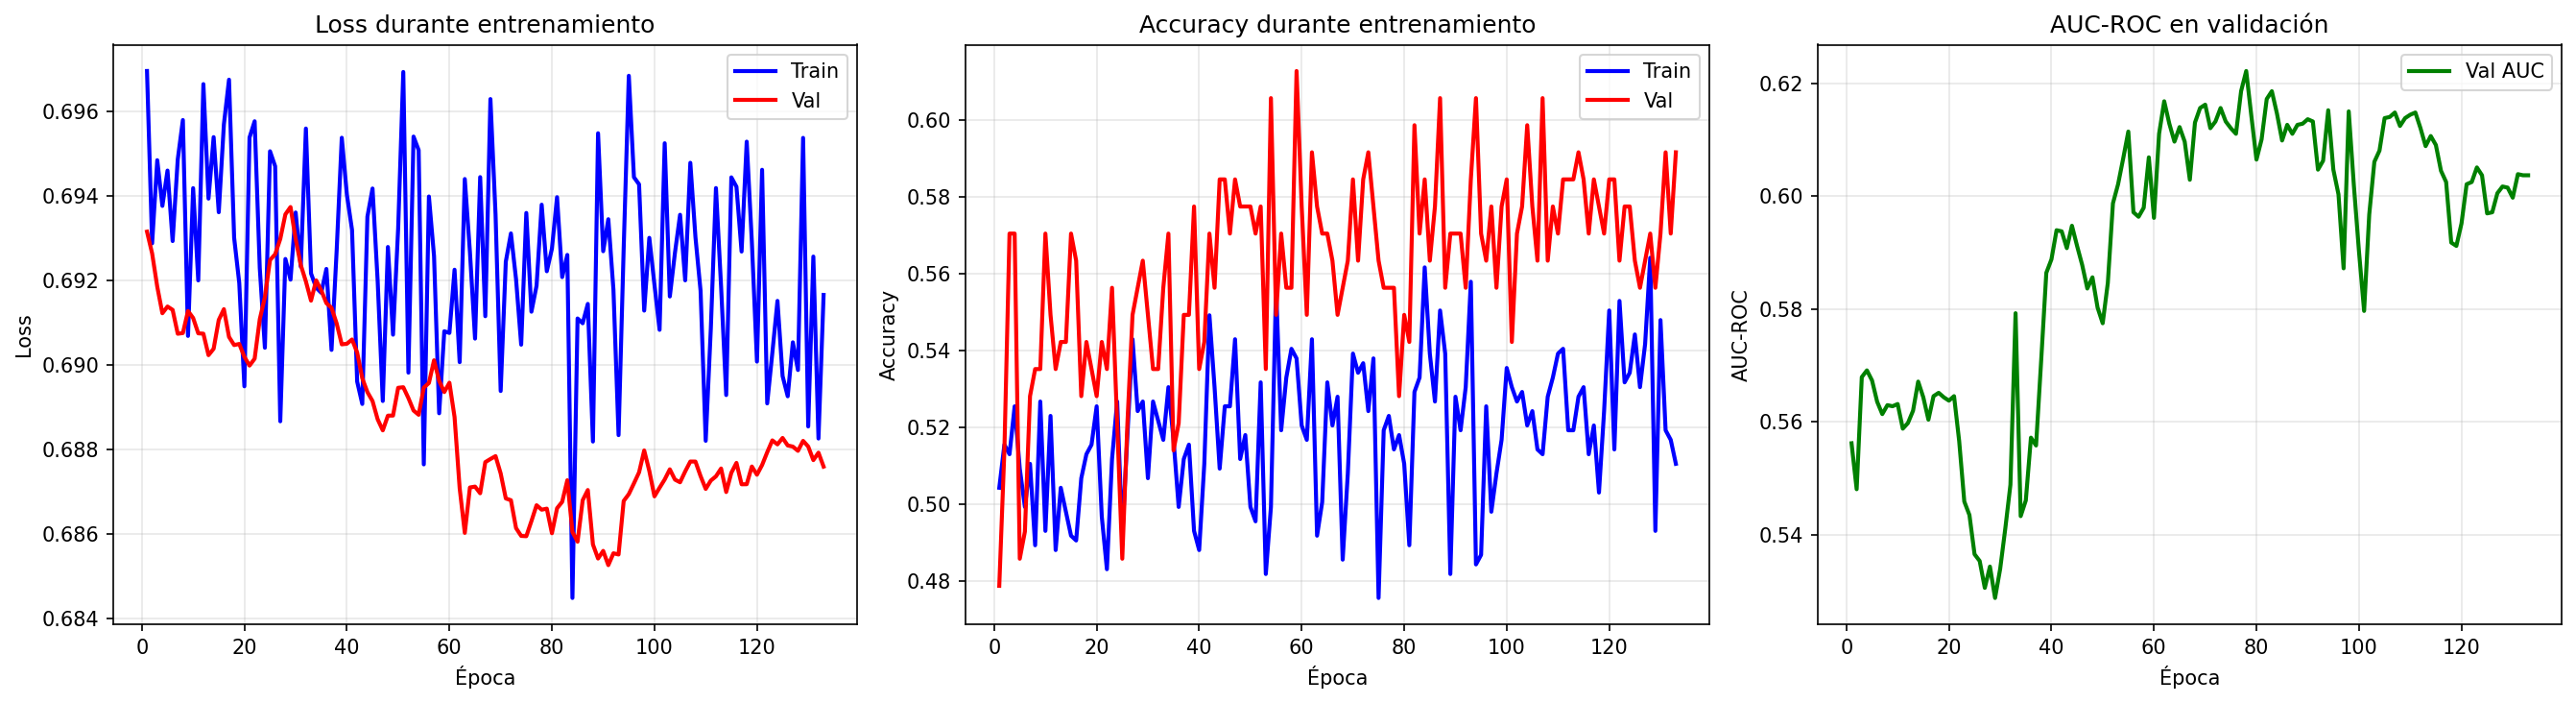
\includegraphics[width=\columnwidth]{training_curves.png}
    \caption{Con DANN ($\alpha\!=\!0.212$)}
  \end{subfigure}
  \caption{Curvas de entrenamiento — Con DANN. Val AUC máximo: 0.622.}
  \label{fig:training}
\end{figure}

\begin{figure}[t]
  \centering
  \begin{subfigure}[b]{0.48\columnwidth}
    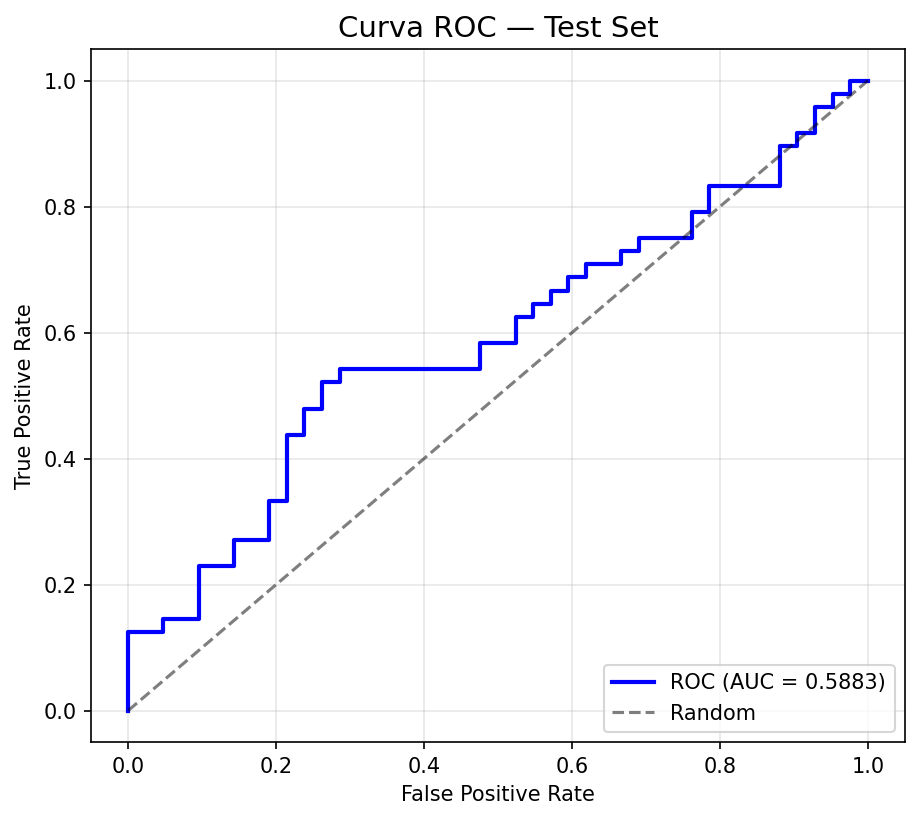
\includegraphics[width=\linewidth]{roc_curve.png}
    \caption{Con DANN (AUC\,=\,0.588)}
  \end{subfigure}\hfill
  \begin{subfigure}[b]{0.48\columnwidth}
    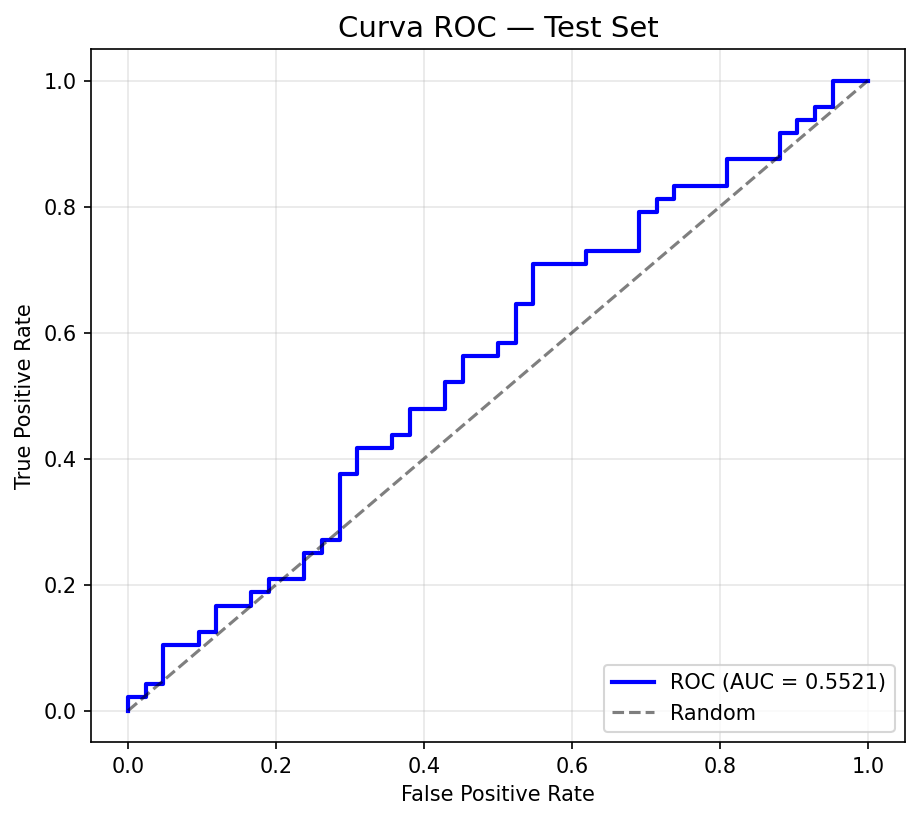
\includegraphics[width=\linewidth]{../results_no_dann/roc_curve.png}
    \caption{Sin DANN (AUC\,=\,0.552)}
  \end{subfigure}
  \caption{Curvas ROC en el conjunto de test (PITT + OLIN, $n\!=\!90$).}
  \label{fig:roc}
\end{figure}

\begin{figure}[t]
  \centering
  \begin{subfigure}[b]{0.48\columnwidth}
    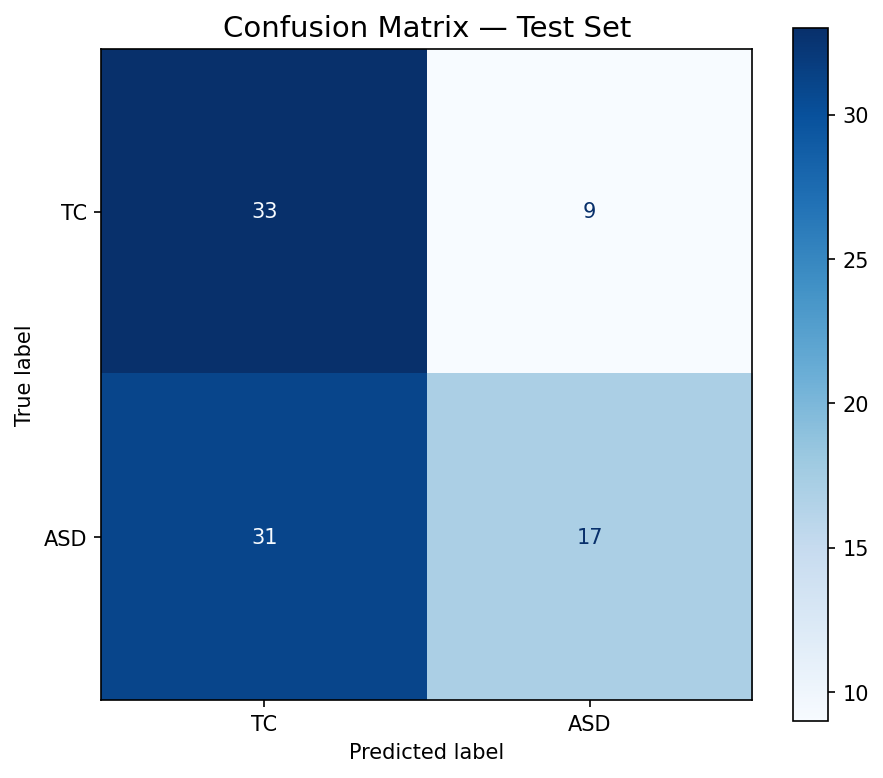
\includegraphics[width=\linewidth]{confusion_matrix.png}
    \caption{Con DANN ($\tau\!=\!0.51$)}
  \end{subfigure}\hfill
  \begin{subfigure}[b]{0.48\columnwidth}
    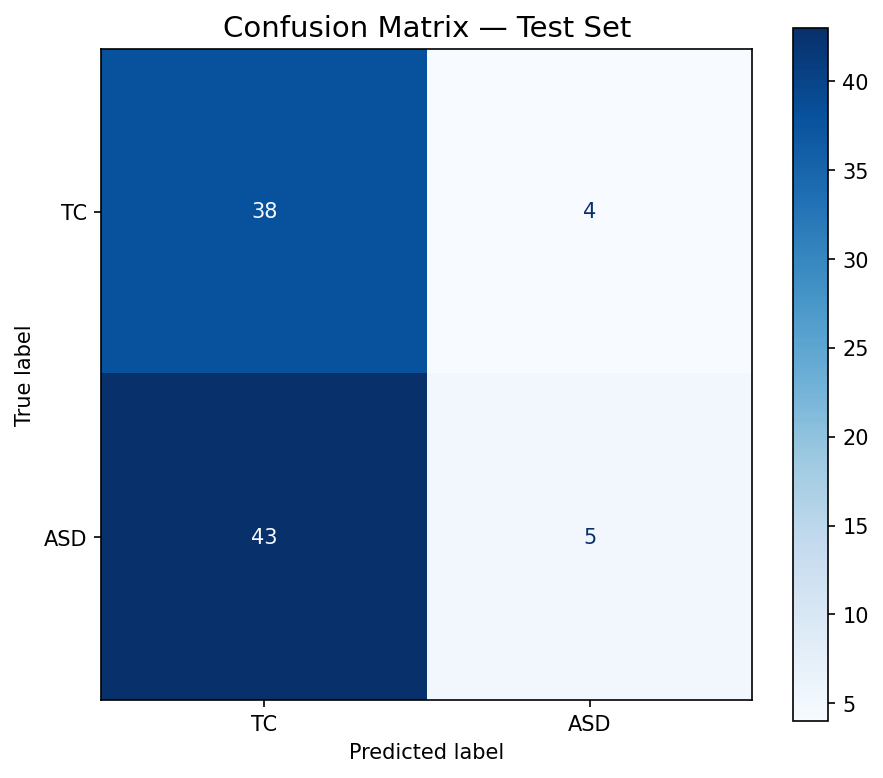
\includegraphics[width=\linewidth]{../results_no_dann/confusion_matrix.png}
    \caption{Sin DANN ($\tau\!=\!0.49$)}
  \end{subfigure}
  \caption{Matrices de confusión con umbral calibrado en validación.}
  \label{fig:conf}
\end{figure}

Con $n^+\!=\!48$, $n^-\!=\!42$, el IC95\% del DANN incluye 0.5
($z\!\approx\!1.47$, $p\!\approx\!0.14$) y la diferencia de 0.036 no
alcanza significancia convencional ($z\!\approx\!0.42$,
$p\!\approx\!0.67$). Esto no invalida los resultados, sino que los
enmarca correctamente: la tendencia favorable de DANN es
\emph{consistente} con la hipótesis pero no la \emph{demuestra}
con el diseño experimental actual.

% ---- 5. Discusión ------------------------------------------------------------
\section{Conclusiones y Trabajo Futuro}

\textbf{AUC\,$\approx$\,0.55--0.59} es coherente con la literatura:
la diferencia ASD--TC en fALFF y ReHo tiene un efecto de tamaño
pequeño~\cite{heinsfeld2018}. Los $|d|\!\approx\!0.08$ del análisis
VBM anticipaban este resultado. 

El modelo con DANN muestra una tendencia favorable en todas las métricas de test (∆AUC = 0.036, ∆balanced accuracy = 6.6 pp). Los AUC cercanos al valor base de 0,5 reflejan la dificultad intrínseca del
problema. Representar el volumen completo en
3D o usar matrices de conectividad (donde la literatura reporta AUC
$\approx$\,0.65) podría aumentar la señal disponible.

\textbf{Trabajo futuro (prioridad alta):}
\begin{itemize}
  \item \emph{Leave-One-Site-Out} (LOSO) + test pareado de DeLong
        para obtener poder estadístico adecuado en la comparación
        DANN vs.\ sin-DANN.
  \item Repetición con múltiples semillas para cuantificar varianza
        del AUC.
  \item CNN 3D directamente sobre tensores NIfTI (sin cuantización
        PNG) para evitar la pérdida de rango dinámico.
  \item Armonización estadística ComBat~\cite{johnson2007} como
        alternativa o complemento al DANN adversarial.
\end{itemize}

% ---- Referencias -------------------------------------------------------------
\bibliographystyle{IEEEtran}
\bibliography{referencias}

\end{document}
